Dans cette section nous appliquons le modèle de transport et
dissolution d'alumine en fonction de la température proposé dans la
section \ref{sec:populations-model} dans le cadre d'une cuve
d'électrolyse industrielle pour déterminer la répartition de l'alumine
dissoute dans le bain de celle-ci. Nous utilisons la cuve AP32, qui
exploite la technologie de cuve d'électrolyse AP
Technology\texttrademark\ développée par RioTinto. Les premières cuves
basées sur la technologie AP ont été mises en production au début des
années 1990, et plus de \num{4000} d'entre elles fonctionnent encore
actuellement en production \cite{RiotintoAP30}. Nous commençons par
présenter le design et le mode d'opération de la cuve AP32. Nous
détaillerons ensuite le choix des différentes données qui
interviennent dans modèle numérique proposé dans la section
\ref{sec:populations-discretisation} et dans le cadre de la cuve
AP32. Finalement, nous présenterons une sélection de résultats
numériques obtenus.


% detail des aspects importants de l'operation d'une cuve
% d'electrolyse:
%  - geometrie de la cuve (taille, nombre d'anodes, epaisseur de bain
%    et de metal,
%  - alimentation electrique
%  - etat stationnaire de l'ecoulement, interface. remarque sur les
%    talus.
%  - control de la concentration d'alumine
%  - schema d'injection periodique, position des injecteurs
%  - calcul de la conductivite sigma du bain
%  - conditions initiales
%  - informations sur le post-processing et la visualisation.

\paragraph{Géométrie de la cuve AP32} La structure de la cuve AP32
occupe au sol une longueur d'environ \num{17} \si{\meter} et une
largeur d'environ \num{7} \si{\meter}. L'ensemble de la structure
s'élève sur environ \num{5} \si{\meter}. La figure
\ref{fig:ap32-geometry} montre la disposition des différents éléments
à l'intérieur de la cuve. Les fluides s'étendent horizontalement sur
environ \num{14} \si{\meter} par \num{3.5} \si{\meter}. L'épaisseur de
la couche d'aluminium liquide (en jaune sur la figure
\ref{fig:ap32-geometry-elements}) en contact avec la cathode est
d'environ \num{17} \si{\centi\meter}, tandis que l'épaisseur maximale
du bain électrolytique, au niveau des canaux entre les blocs
anodiques, est d'environ \num{20} \si{\centi\meter}. La figure
\ref{fig:ap32-geometry-electrolyte} illustre le volume occupé par le
bain dans lequel on s'intéresse à la concentration d'alumine, en
orange. Les indentation rectangulaire à la surface de celui-ci
correspondent au volume occupé par les anodes partiellement
immergées. L'ACD est typiquement de l'ordre de \num{3}
\si{\centi\meter}. Ces différentes épaisseurs varient d'un point à
l'autre de la cuve à cause des écoulements dans les fluides, de la
déformation de l'interface bain-métal et des irrégularités à la
surface des anodes. De plus, le volume de métal liquide varie
constamment, d'une part à cause du produit de la réaction
d'électrolyse, et d'autre part à cause des opérations de siphonnage du
métal, qui interviennent environ une fois par jour.

\begin{figure}[t]
  \begin{center}
    \begin{subfigure}[b]{0.49\textwidth}
      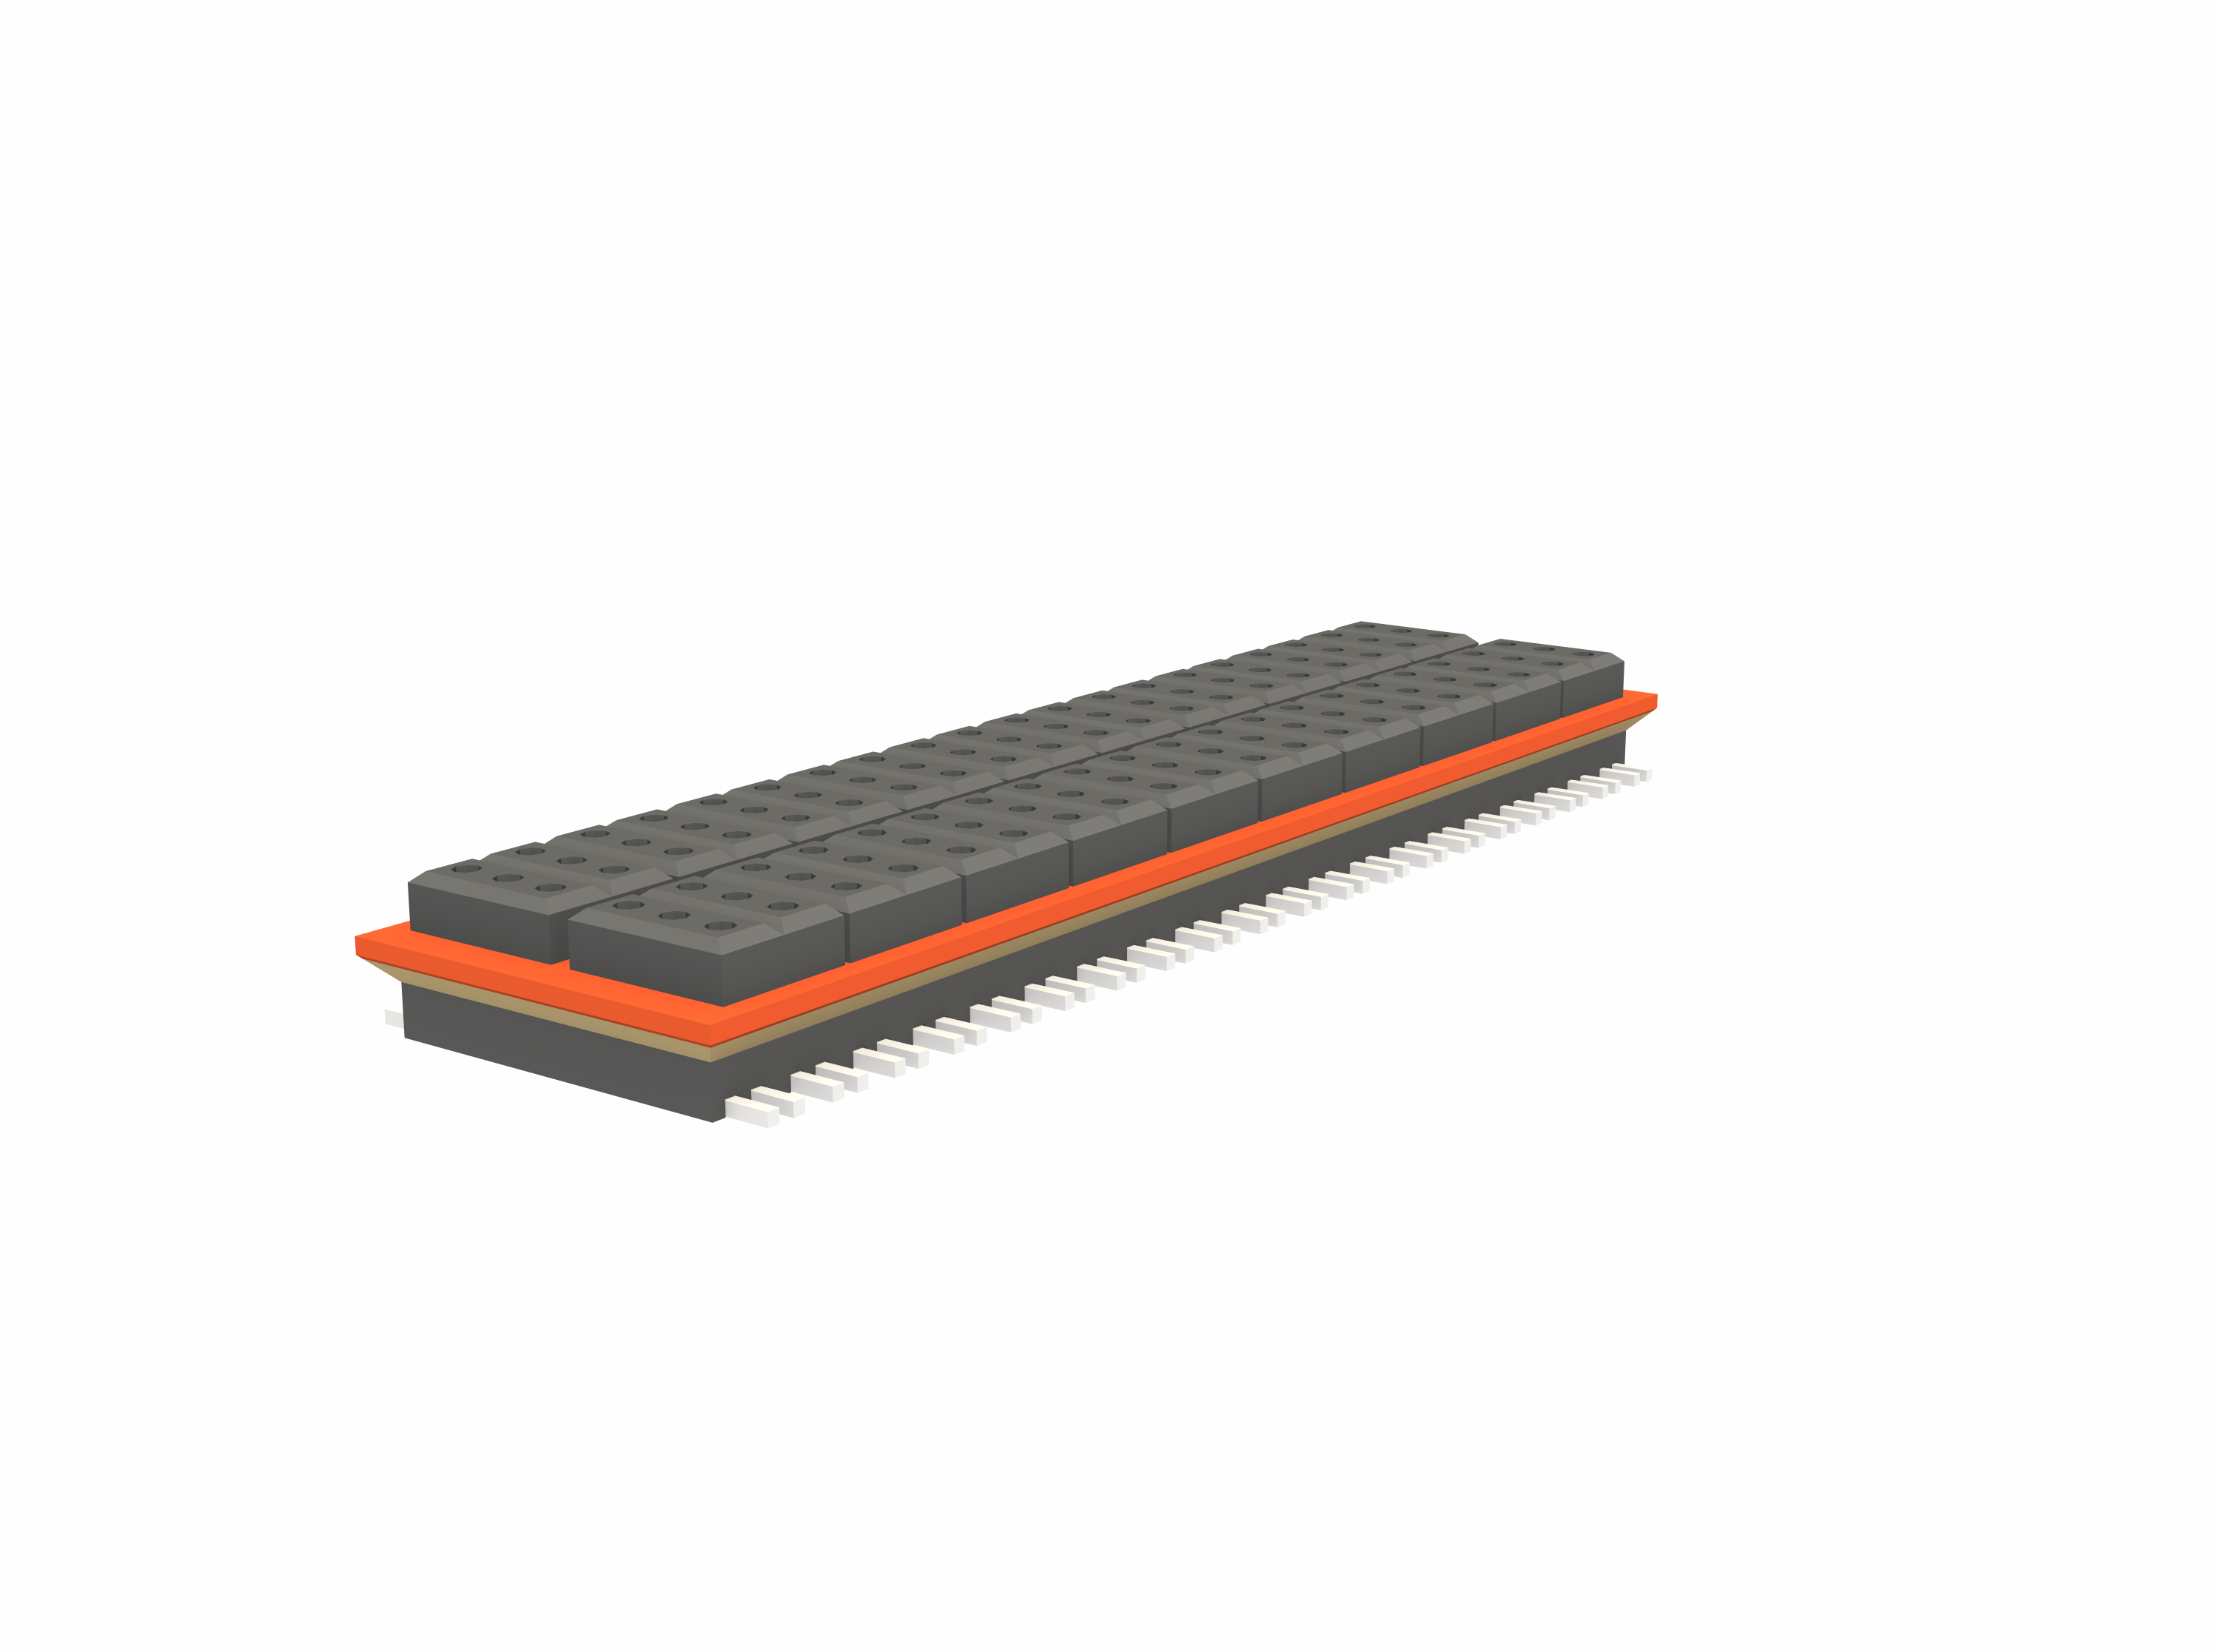
\includegraphics[width=\textwidth]{../media/populations/ap32-mesh-components/print/metal-bath-anodes-cathode-bus-bars.png}
      \caption{Éléments à proximité des fluides}
      \label{fig:ap32-geometry-elements}
    \end{subfigure}

    \begin{subfigure}[b]{0.49\textwidth}
      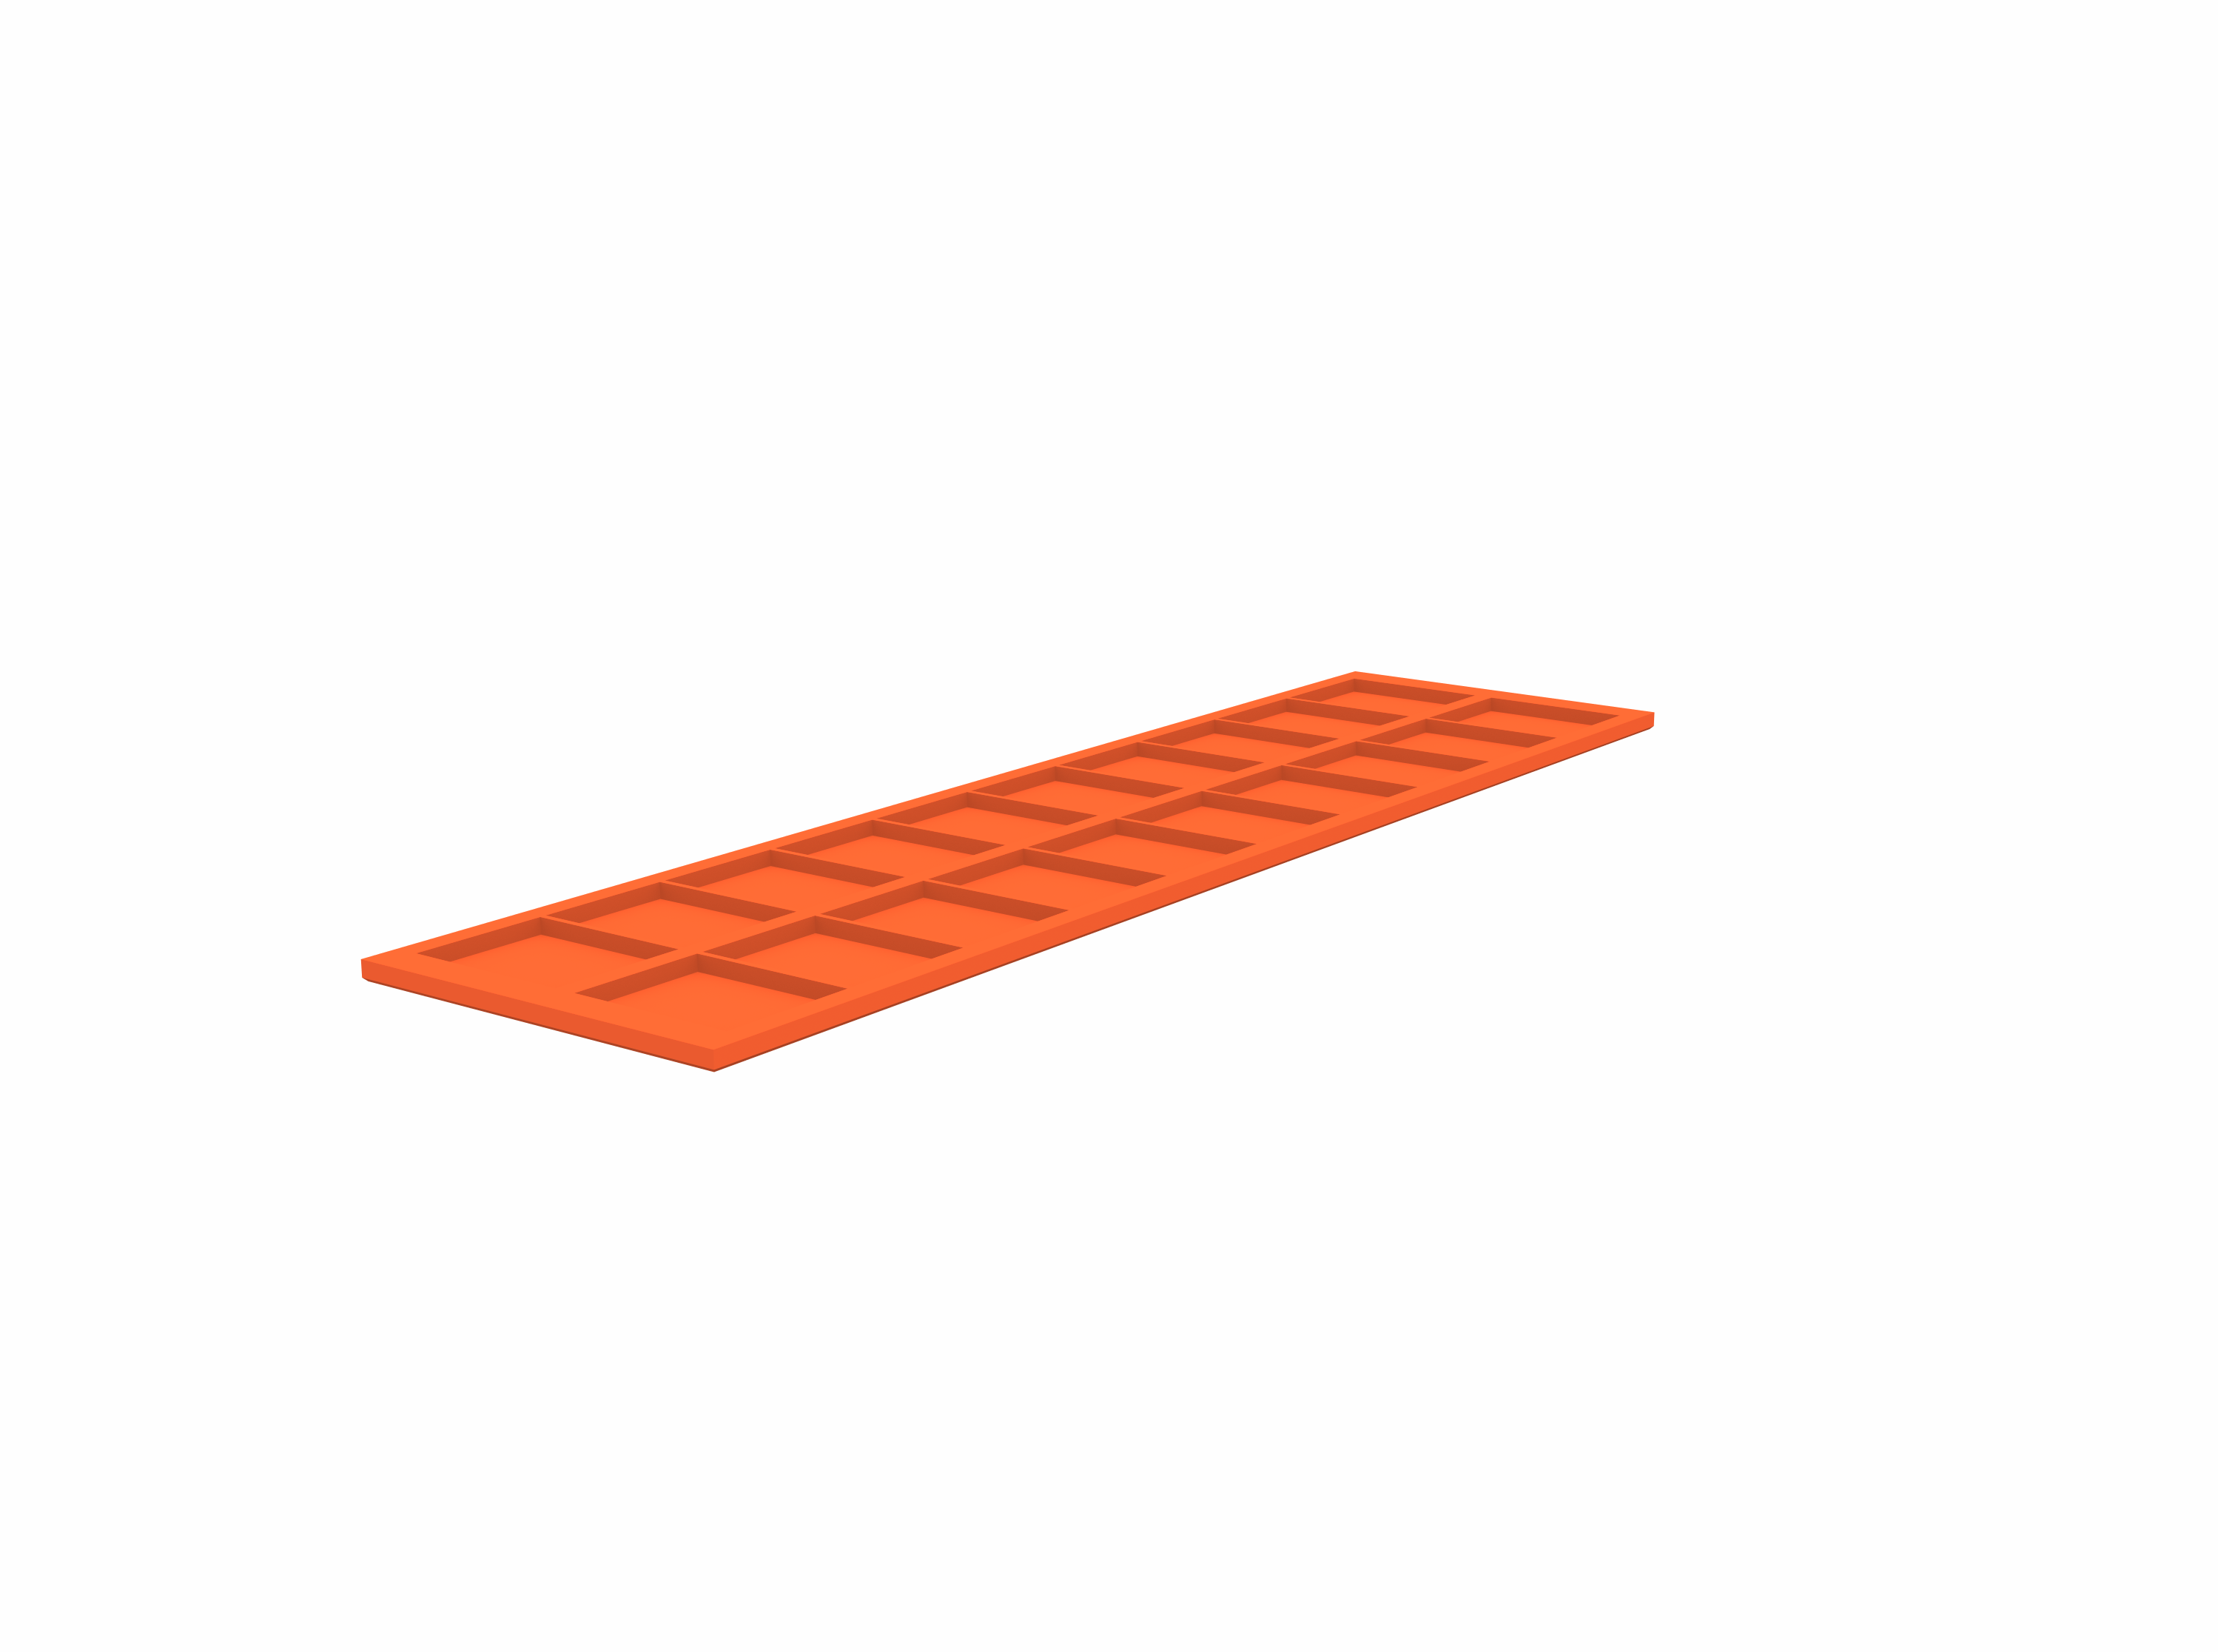
\includegraphics[width=\textwidth]{../media/populations/ap32-mesh-components/print/bath.png}
      \caption{Bain électrolytique}
      \label{fig:ap32-geometry-electrolyte}
    \end{subfigure}

    \caption{Géométrie des éléments importants à proximité
      du bain électrolytique dans une cuve AP32
      (fig. \ref{fig:ap32-geometry-elements}), et détail du volume
      occupé par le bain électrolytique dans cette même cuve
      (fig. \ref{fig:ap32-geometry-electrolyte}). On distingue les
      les anodes en haut et la cathode
      en bas (\textbf{noir}), le bain électrolytique
      (\textbf{orange}), le métal liquide (\textbf{jaune}) et les
      bus bar (\textbf{gris clair}).}
    \label{fig:ap32-geometry}
  \end{center}
\end{figure}

Le plan anodique est composée de deux rangées de 10 anodes chacune,
représentées en noir sur la figure \ref{fig:ap32-geometry-elements}. La
surface du plan anodique est d'environ \num{40.3} \si{\square\meter}
et seulement \num{25}\% de la surface du bain est libre, le reste
étant recouvert par les anodes. La cuve est conçu pour que
l'électrolyte soit traversé par un courant électrique total $I = $
\num{320000} \si{\ampere}, ce qui correspond à une densité de courant
d'environ \num{0.8} \si{\ampere\per\square\centi\meter} à la surface
des anodes. En supposant un rendement de réaction de \num{100}\%, ce
courant électrique permet de réduire par électrolyse \num{29.8}
\si{\gram\per\second} ou \num{2577.1} \si{\kilo\gram} par jour
d'aluminium métallique, \ie, un peu plus qu'\num{1} \si{\cubic\meter}
de métal par jour. Cet accroissement de volume de métal correspond à
une variation de l'épaisseur du métal liquide d'environ \num{2}
\si{\centi\meter}.

Du coté des anodes, la réaction d'électrolyse produit environ
\num{0.8} \si{\mol\per\second} d'oxygène \ce{O2}. Cet oxygène réagit
immédiatement avec le carbone de l'anode pour former du \ce{CO2}. Dans
l'ensemble de la cuve, l'électrolyse produit au total environ \num{80}
\si{\liter} par seconde de gaz, qui remonte vers la surface du bain
par le canal central et les canaux latéraux. La réaction de l'oxygène
avec le carbone des anodes provoque l'érosion de celles-ci à une
vitesse d'environ \num{1100} \si{\kilo\gram} par jour. Étant donné le
nombre total d'anodes et leur taille respectives, chaque anode d'une
cuve AP32 a une durée de vie d'environ 30 jours, après quoi elle doit
être remplacée par une anode neuve.

Pour compenser l'alumine dissoute qui est consommée par la réaction
d'électrolyse, il faut injecter en moyenne au cours du temps $56.3$
\si{\gram\per\second} de poudre d'alumine. Comme déjà mentionné
dans la section \ref{sec:introduction-hall-heroult}, la poudre
d'alumine est déposée à la surface du bain dans le canal central par
une série d'injecteurs dont la position est fixe. Un piqueur vient
percer mécaniquement un trou dans la croûte et créer un accès à la
surface libre du bain avant chaque injection. Ce trou se rebouche
rapidement, et pour cette raison l'injection d'alumine ne peut pas
avoir lieu continûment.

Pour maintenir un rendement maximum, éviter l'émission de gaz
fluorés et minimiser le nombre d'effets d'anodes, il est crucial que
la concentration d'oxyde d'aluminium dissout dans le bain soit
maintenu dans un intervalle très précis. Malheureusement, pour de
nombreuses raisons il est impossible de maintenir un bilan précis de
la quantité d'alumine dans le bain en fonction de ce qui est injecté
et de ce qui est consommé. En effet, l'environnement rend difficile la
pesée précise des quantités déposées, une partie des particules
volatiles ne parviennent jamais dans le bain, des agrégats se forme,
dont une partie s'accumule au fond de la cuve sur la cathode, et des
réactions chimiques parasites viennent, entre autres, grever ce bilan.

Pour contourner cette difficulté, les opérateurs exploitent le fait
que la resistivité du bain électrolytique dépend de la concentration
d'alumine dissoute, et atteint un minimum à la concentration optimale
$\csat \approx$ \num{3}\% masse. En mesurant la chute de potentiel
électrique à travers le bain électrolytique, on maintient la
concentration d'alumine dissoute au voisinage de la concentration
optimale en alternant une phase de sur-alimentation en alumine et une
phase de sous-alimentation. Durant la phase de sur-alimentation, la
concentration d'alumine va passer au-delà de la concentration optimale
par conséquent accroître la resistivité du bain. Passé un certain
seuil, on débute une phase de sous-alimentation, durant laquelle la
résistivité commence par chuter, puis croît à nouveau. Passé un
certain seuil, on amorce une phase de sur-alimentation, et ainsi de
suite.

Dans chacune des phase de sur-alimentation ou sous-alimentation, les
injecteurs déposent les doses d'alumine selon une cadence préétablie
et périodique. La période et une taille des doses peut être spécifiée
indépendemment pour chaque injecteur.

\begin{figure}[t]
  \begin{center}
    \begin{tikzpicture}
      \begin{axis}[
          hide axis,
          colorbar,
          scale only axis,
          height=0.41\rasterimagewidth,,
          width=\rasterimagewidth,
          colorbar horizontal,
          point meta min=0.00,
          point meta max=0.05,
          colorbar style={
            title=Vitesse $u$ [\si{\meter\per\second}],
            width=7.4cm,
            height=0.3cm,
            xtick={0.00, 0.01, 0.02, 0.03, 0.04, 0.05},
            xticklabel style={
              /pgf/number format/fixed,
              /pgf/number format/fixed zerofill,
              /pgf/number format/precision=2
            },
            scaled x ticks = false,
            at={(0.5\rasterimagewidth,0.4cm)},
            anchor=north
          }
        ]
        \addplot [] coordinates {(0,0)};
        \node (myfirstpic) at (0,0) {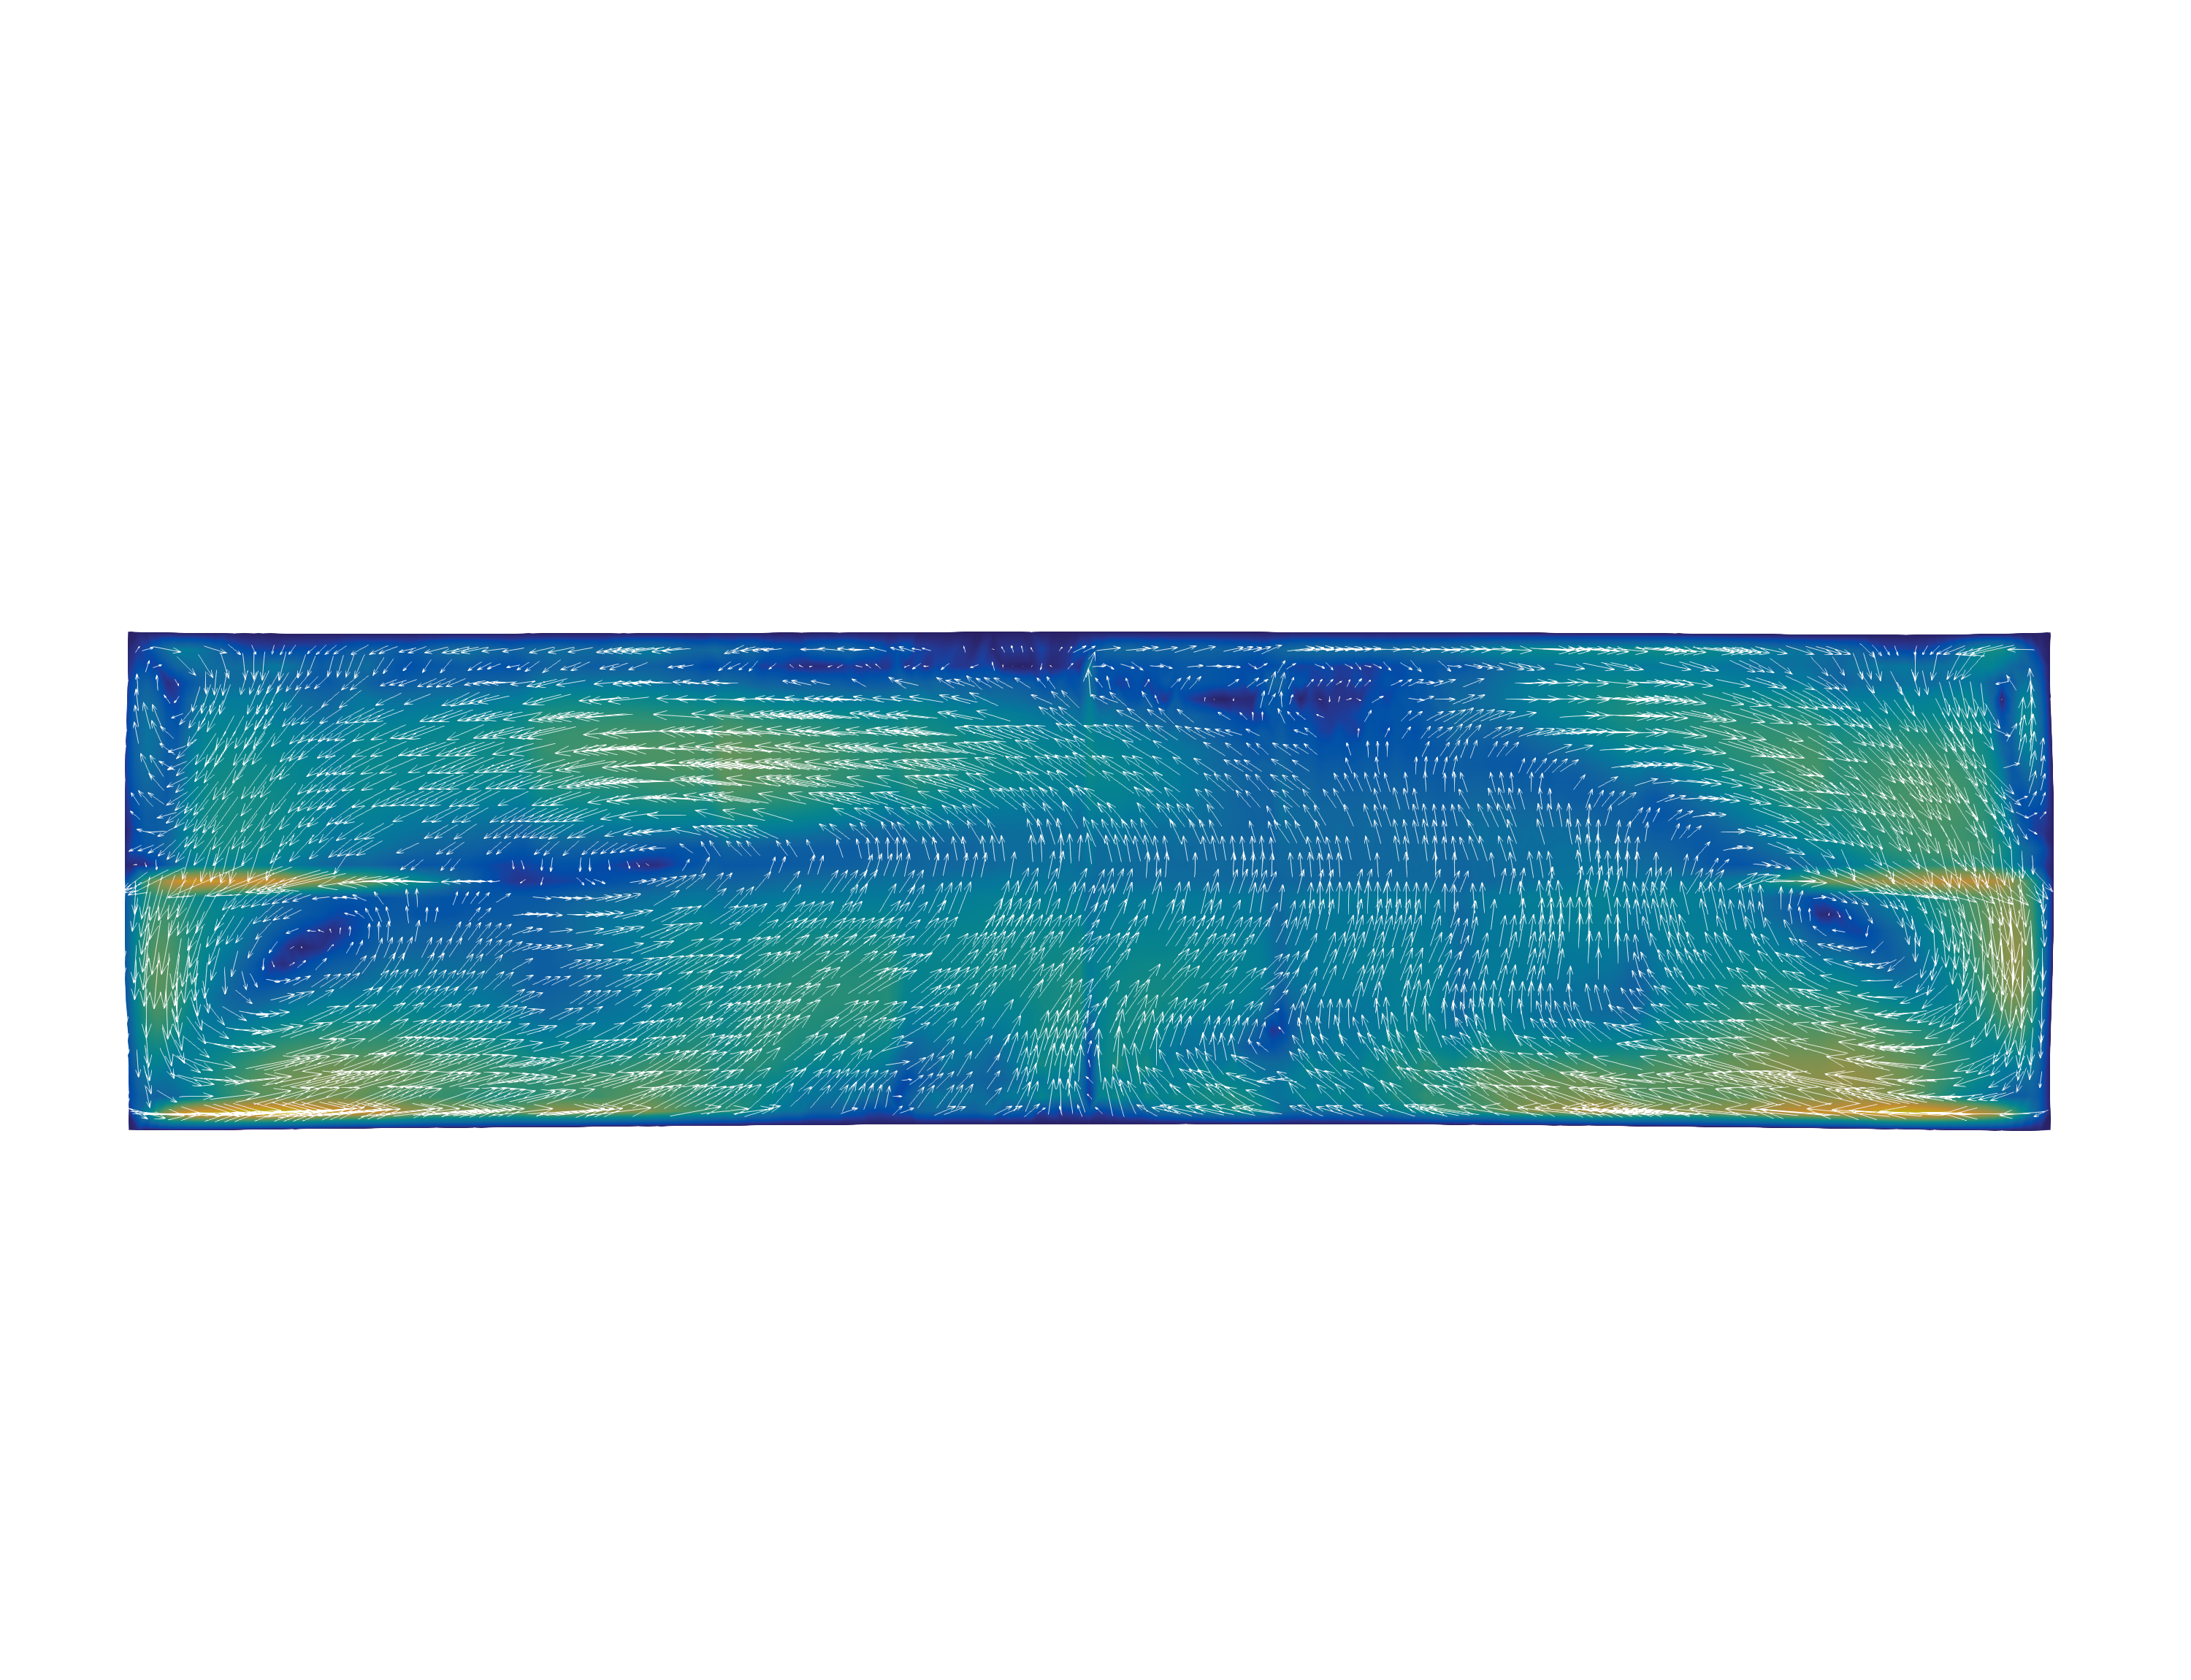
\includegraphics[width=\rasterimagewidth]{{../media/populations/ap32-fluid-flow/print/acd-all-anodes-velocity-0.00-0.05}.png}};
      \end{axis}
    \end{tikzpicture}
    \caption{Champ de vitesse $u$ dans le bain électrolytique d'une
      cuve AP32 restreint sur une surface placée à mi-hauteur de
      l'ACD, vue depuis dessus. Cette situation correspond à un état
      d'opération standard.}
    \label{fig:ap32-flow-acd}
  \end{center}
\end{figure}

\begin{figure}[t]
  \begin{center}
    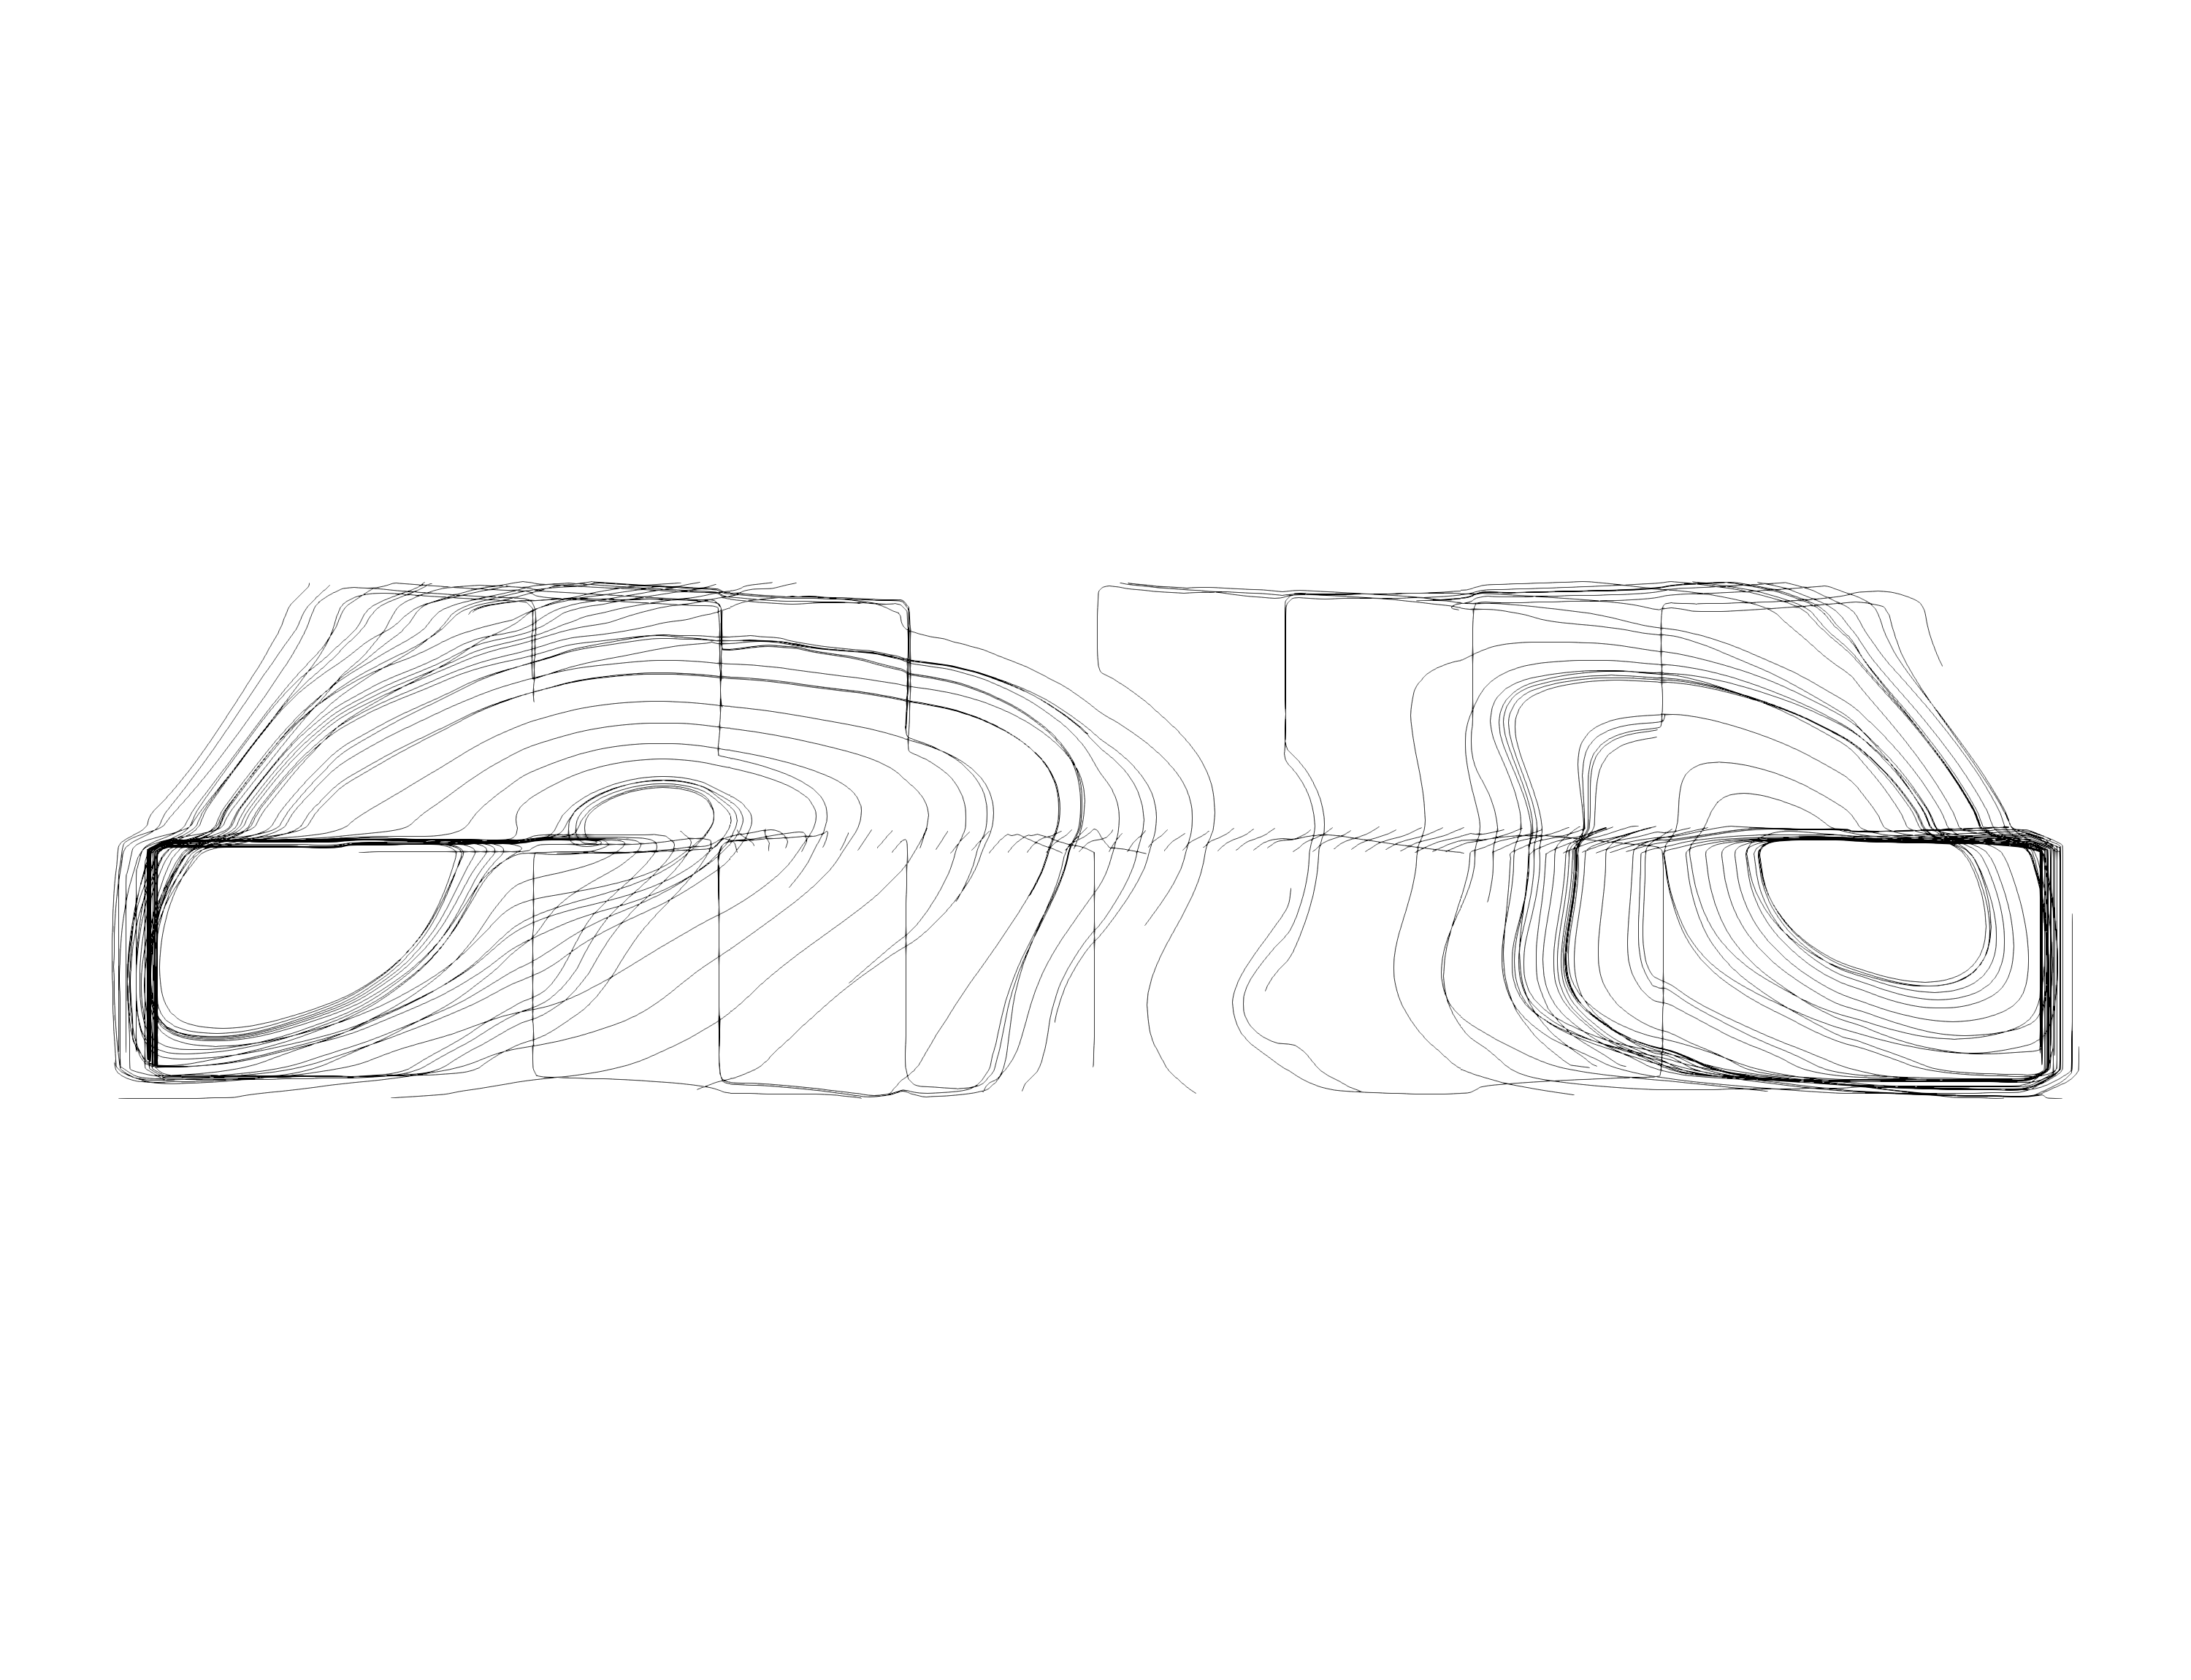
\includegraphics[width=\rasterimagewidth]{../media/populations/ap32-fluid-flow/print/chanel-velocity-streamlines.png}
    \caption{Lignes de courant correspondant au champ de vitesse
      représenté sur la figure \ref{fig:ap32-flow-acd}. Les lignes de
      courant prennent leur origine le long du canal central.}
    \label{fig:ap32-flow-streamlines}
  \end{center}
\end{figure}

\paragraph{Calcul de l'écoulement dans le bain} Une approximation de vitesse
d'écoulement du bain $u$ et de la densité de courant $j$ dans la cuve
AP32 est obtenue par l'intermédiaire du modèle multiphysique
stationnaire proposé par S. Steiner \cite{Steiner2009}, J. Rochat
\cite{Rochat2016} déjà introduit dans la section
\ref{sec:populations-introduction}. La figure \ref{fig:ap32-flow-acd}
représente la vitesse d'écoulement ainsi calculée par le logiciel
Alucell dans le bain électrolytique de la cuve AP32, dans
l'ACD. L'écoulement dans les fluides forme deux tourbillons principaux
qui tournent en sens opposés. Deux petits tourbillons se forment dans
les coins avals. Les vitesse maximales de l'écoulement (\num{5}
\si{\centi\meter\per\second} environ) sont atteinte dans le canal
central au niveau des extrémités de la cuve, ainsi que le long de la
parois amont, de part et d'autre de la cuve. Dans le reste du bain et
en particulier sous les anodes la vitesse d'écoulement dépasse
rarement \num{2} \si{\centi\meter\per\second}. La figure
\ref{fig:ap32-flow-streamlines} illustre les lignes de courant de
l'écoulement dans le bain. On remarque les lignes de courant
s'engagent volontiers dans les canaux latéraux et dans le bain en
pourtour des rangées d'anodes.

\paragraph{Conditions initiales et paramètres du modèle}
% concentration initiale, température initiale
% paramètres numérique. (deltat, maillage, deltar, N_r)
% injections
% parametres physiques, parametres du modele
% calcul du coefficient de diffusion

% Ne pas oublier: S_k, \tau_k, D_c, D_\temperature, \sigma, N et T.


\begin{table}
  \begin{center}
    \caption{Paramètres physiques qui interviennent dans la chute
      d'une particule d'alumine dans un bain électrolytique.}
    \label{tab:fall-physical-parameters}
    \begin{tabularx}{\textwidth}{@{}lllX@{}}
      \toprule
      Quantité                         & Valeur        & Unités                                      & Description \\
      \midrule
      $\electrolytedensity$            & \num{2130}    & \si{\kg\per\cubic\meter}                    & Masse volumique du bain électrolytique           \\
      $\aluminadensity$                & \num{3960}    & \si{\kg\per\cubic\meter}                    & Masse volumique de l'oxyde d'aluminium           \\
      $\electrolytehc$                 & \num{2130}    & \si{\kg\per\cubic\meter}                    & Chaleur spécifique du bain électrolytique        \\
      $\aluminahc$                     & \num{3960}    & \si{\kg\per\cubic\meter}                    & Chaleur spécifique de l'oxyde d'aluminium        \\
      $g$                              & \num{9.81}    & \si{\meter\per\square\second}               & Accélération de la gravité terrestre             \\
      $I$                              & \num{320000}  & \si{\ampere}                                & Courant électrique total                         \\\relax
      [\ce{Al2O3}]                     & \num{0.102}   & \si{\kilo\gram\per\mol}                     & Masse molaire de l'oxyde d'aluminium             \\
      $\tinit$                         & \num{0}       & \si{\kelvin}                                & Température initiale du bain électrolytique      \\
      $\tinj$                          & \num{0}       & \si{\kelvin}                                & Température d'injection des particules d'alumine \\
      $\aluminadissolutionenthalpy$    & \num{0}       & \si{\joule\per\kilo\gram\per}               & Enthalpie de dissolution de l'oxyde d'aluminium  \\
      $\conductivity$                  & \num{0}       & \si{\siemens\per\meter}                     & Conductivité électrique du bain électrolytique   \\
      $\electrolytelaminarviscosity$   & \num{2e-3}    & \si{\kilo\gram\per\meter\per\second}        & Viscosité laminaire du bain électrolytique       \\
      $\electrolyteturbulentviscosity$ & \num{2e-3}    & \si{\kilo\gram\per\meter\per\second}        & Viscosité turbulente du bain électrolytique      \\
      \bottomrule
    \end{tabularx}
  \end{center}
\end{table}
